\documentclass{article}

\usepackage[english]{babel}
\usepackage[letterpaper,top=2cm,bottom=2cm,left=3cm,right=3cm,marginparwidth=1.75cm]{geometry}
\usepackage{amsmath}
\usepackage{amsfonts}
\usepackage{amssymb}
\usepackage{algorithm} 
\usepackage{algpseudocode} 
\usepackage{graphicx}
\usepackage[colorlinks=true, allcolors=blue]{hyperref}

\title{AAGT Homework $\#3$}
\author{Jakub Grondziowski}
\date{}

\begin{document}
\maketitle

\section{Task a}
On the below examples I assume that dots are representations of Eve's vertices, and that Eve wants to see even priorities infinitely often. \\

Example of a game where staying in a winning region is not enough for Eve to win:
\begin{figure}[h]
\centering
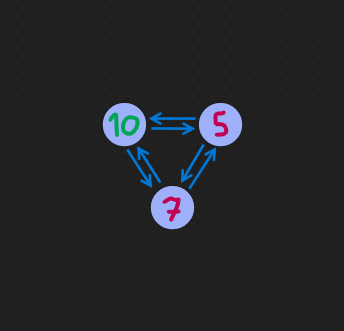
\includegraphics[width=0.4\textwidth]{bad.png}
\caption{\label{fig:counter}Eve can alternate between 5 and 7, assuring she won't win, even though she could.}
\end{figure}

Example of a game where staying in a winning region is enough for Eve to win:
\begin{figure}[h]
\centering
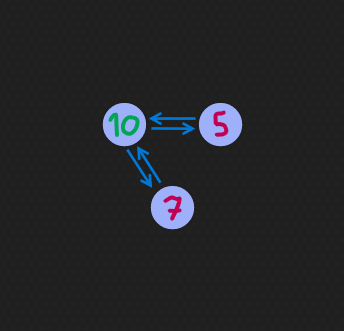
\includegraphics[width=0.4\textwidth]{good.png}
\caption{\label{fig:counter}Every other move will lead to a larger, even priority.}
\end{figure}

In both cases the whole graph is a winning region for Eve - she can always assure to visit a node denoted with 10 on every other move. The difference being that she cannot assure to do that by picking a positional strategy at random in the first case.

\section{Task b}

I will try to reduce the easy game problem to solving parity game problem. First of all I'll explain in more details the exact condition that must be met for the game to be easy for Eve. For any Eve's winning region she must be able to pick a random strategy and still manage to win every time. The random strategy cannot exit the winning region of Eve. We can confront this fact with the winning condition of parity game - Eve wants to see an even priority infinitely many times. Winning regions of parity games must have at least one loop that allows that. If the winning region does not have a loop, there is no way to assure that condition is met, since eventually the player would exit the region. We know that Eve won't leave the winning region if she is in one - that means that her only way of losing at this point is choosing some wrong edges with odd priorities. That leads us to the conclusion of when the parity game is not easy for Eve - if there exists a cycle, whose path creates a word with the largest priority being odd, then Eve can lose a parity game if her random strategy involves picking this exact cycle over and over again. That naturally creates the condition that must be met for the game to be easy for Eve - there mustn't be any cycle inside her winning region whose largest priority of the cycle path is odd. It makes more sense if we look at it from more general point of view - Eve cannot lose if every cycle that she finds herself in gives the path with largest priority being even. There may be some edges with a larger odd priority - but since they're not in any cycle they will be visited finitely many times and thus are not an issue. \\

We can start our reduction from asking our oracle (which in my case is solving parity game) about the winning region of Eve. If the winning region is empty, then the game is paradoxically easy for Eve, since there are no nodes in set $W_{E} \cap Pos_{E}$. If it's not, we need to calculate all possible cycles with no repeated node on the path. That way we avoid the processing of cycles that are just a set of smaller cycles glued together (of course if Eve uses such a cycle then everything is still fine, since every such cycle can be described as a sum of smaller cycles with no repeating nodes). In order to find all cycles with no repeating nodes we can, for example, use Johnson's algorithm, which has a running time of $O((n + e)(c + 1))$, where $n$ is the size of the graph, $e$ is number of edges and $c$ is the number of elementary circuits in the graph. Note that we run this algorithm on Eve's winning region only.\\

Now we must find the maximal priorities for every cycle that we've found. If maximal priority of every cycle is even, the game is easy for Eve. If there is one or more cycles whose maximal priority is odd, the game is not easy for Eve. The running time of determining all maximums is in its worst case $O(e * n)$, since even if there are a lot of cycles (big or small), there will never be more than $e$ of them. Finding maximum of a given array (in our case, cycle) of priorities is linear, and since the priorities reside in the vertices, calculating one maximum will take at max $n$ steps. \\

Using the solving parity game problem as oracle we've shown that the easy game problem can be solved using a polynomial time algorithm. This concludes the proof.

\end{document}